The results depicted in Figure~\ref{fig:wave_scattering_results} illustrate the scattering of the scalar field $\Phi$ by the GW150914 binary black hole merger system at three distinct moments in time. Panel \textbf{A} corresponds to $t = 0$, panel \textbf{B} represents $t = 8.811$, and panel \textbf{C} corresponds to $t = 55.068$.

Following the initial interaction, the black holes generate a wavefront in a pattern resembling a cardioid, where the cusp coincides with the hole location and propagates in alternating directions. This shape resembles that observed in wave scattering by a single black Schwarzschild hole (See Figs. 5 and 7 of Ref.~\cite{PhysRevD.84.104002}), however, in the case of a merging binary, we can observe clear effects arising from the rotation of the holes and interference from the waves produced by each. An animation of the scattering process can be viewed in this thesis repository, Ref.~\cite{ThesisRepo} under \texttt{img/wave\_scattering/scattering.gif}.

%Frames used: 0 7 19
\begin{figure}[h]
  \centering
  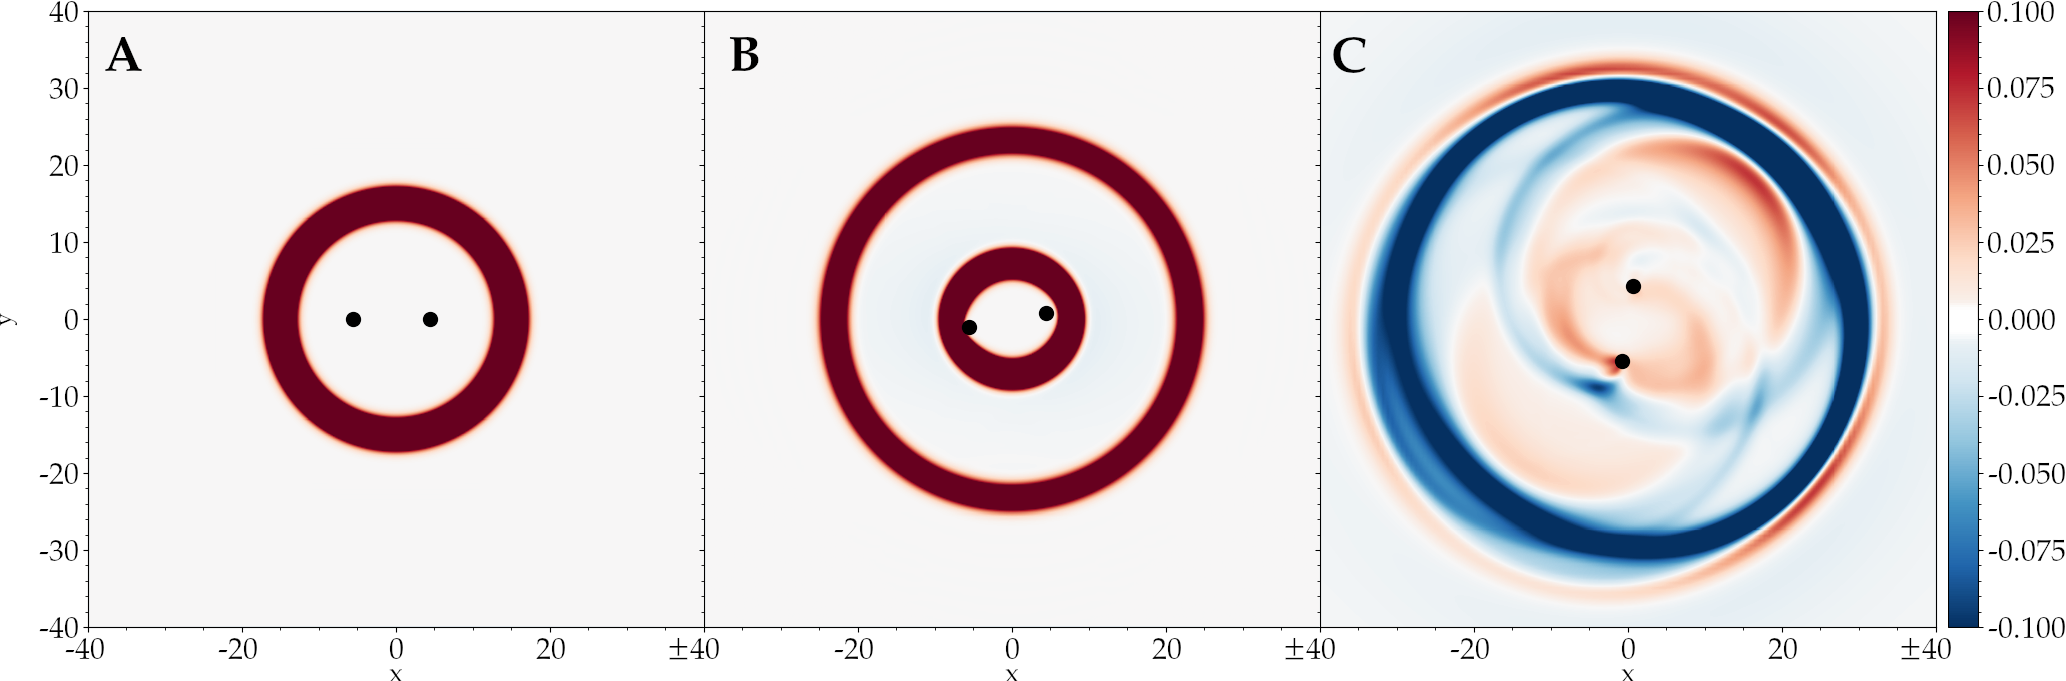
\includegraphics[width=\linewidth]{img/wave_scattering/scattering_frames}
  \caption{Scalar field $\Phi$ scattering of the GW150914 binary merger in three moments in time. Panel \textbf{A} corresponds to $t = 0$, panel \textbf{B} represents $t = 8.811$, and panel \textbf{C} corresponds to $t = 55.068$.}
  \label{fig:wave_scattering_results}
\end{figure}

In addition to pure field values, we have, as was previously mentioned, extracted the multipolar components of the field at various radii during the simulation. For clarity, we will focus on the $l=2,m=0$ component of the field at a radius of $40$ in this discussion.

The plot in the top left panel of Fig.~\ref{fig:multipolar_plots} shows the field value as a function of time. The signal has a ``blip'' between $t=0$ and $t=50$ due to the fact that our multipolar Gaussian initial data splits in half at $t=0$, resulting in an outgoing component of the initial data the gets detected first by the decomposition. After $t=50$, we observe a nonlinear signal resulting from the field's interaction with the binary, which settles down after a number of oscillations.

It is also useful to analyze the logarithm of the absolute value of the field in order to identify regions where quasinormal ringdown might be taking place. This is what can be seen in the top right plot of Fig.~\ref{fig:multipolar_plots} between approximately $t=60$ to $140$. Additionally, in order to better visualize this decaying oscillation, we plot on the bottom panels of Fig.~\ref{fig:multipolar_plots} the same quantities as described on the top panels but in between $t=67.2$ and $t=136.5$. Even tough the signal is clearly oscillating in a damped manner, it is difficult to identify the shape of the plot of the bottom right panel to the classical shape of the quasinormal ringdown. There are very prominent deformations on the shapes of the oscillation ``crests'' and at times their periods seem to be of variable size.

\begin{figure}[h]
  \centering
  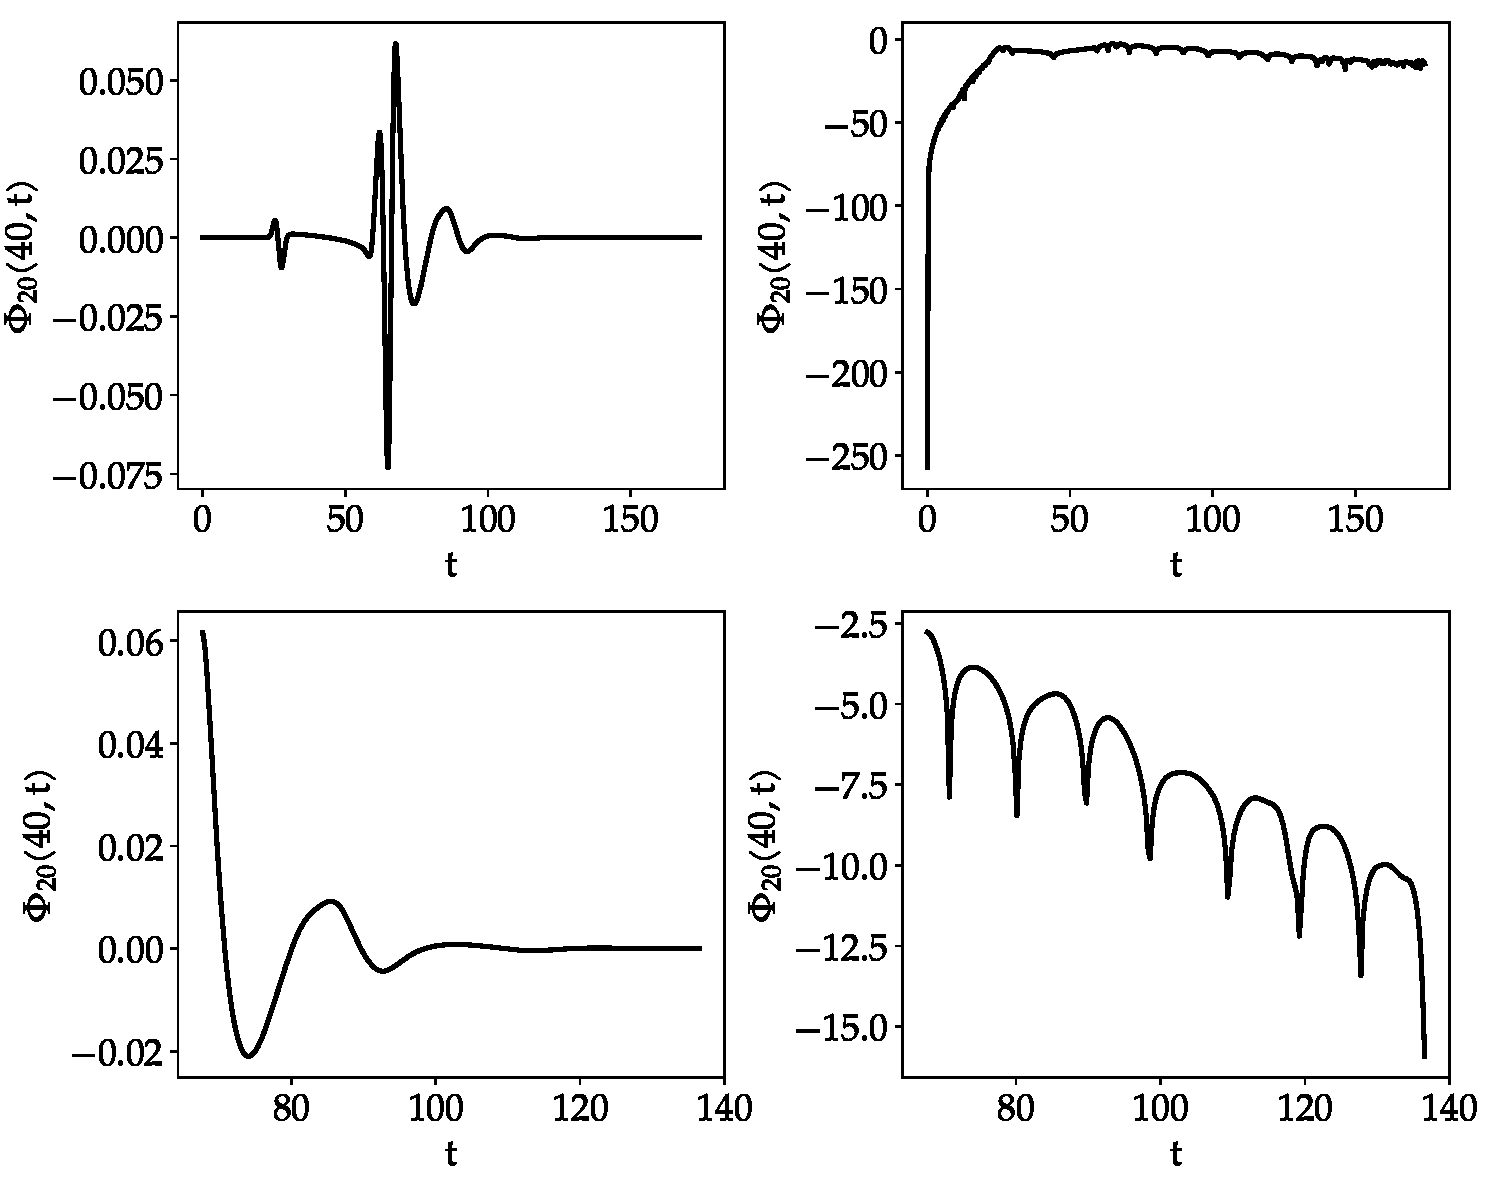
\includegraphics[width=\linewidth]{img/wave_scattering/multipolar_plots}
  \caption{Top panels: Plot of the multipolar field component $l=2,m=0$ at $r=40$ for the whole simulation time. Bottom panels: Same quantities as in the top panels but restricted to the $t=[67.2, 136.5]$ time period. The right panels plot the logarithm of the absolute value of the field.}
  \label{fig:multipolar_plots}
\end{figure}

The departure from the quasi-normal ringdown is more noticeable when attempting to fit the classical quasi-normal model, $A \exp(-\omega_i t) \cos(\omega_r t + \phi)$, to the data between $t=67.2$ and $t=136.5$. The left plot of Fig.~\ref{fig:multipolar_plots_fit} shows the residual of the fitting, i.e., the absolute value of the difference between the simulated data and the data obtained by substituting the fit parameters back into the model. Despite the quasi-normal ringdown model not agreeing well with the simulated data, the fitted frequency parameters are presented on the left plot for completeness.

This discussion requires additional attention. The topic of modeling quasinormal modes by fitting data to wave signals is a complex matter. In particular, determining the number of modes to fit (i.e., whether to fit overtones) and selecting a starting time for fitting may result in varying levels of agreement and different outcomes for quasinormal frequencies. These aspects have recently been extensively studied, as reported in Refs.~\cite{PhysRevD.101.104005, ota2022black} and works therein. Moreover, recent developments suggest that neglecting nonlinear behavior in ringdown analysis, as argued in Ref.~\cite{PhysRevLett.130.081401}, is indeed incorrect.

We emphasize that the results presented in this section are preliminary and primarily illustrative. We do not intend to make any claims or rigorous assertions about the nature of quasinormal modes. Additionally, we have opted to employ a standard linear quasinormal mode model to extract fundamental information from our simulated data.

\begin{figure}[h]
  \centering
  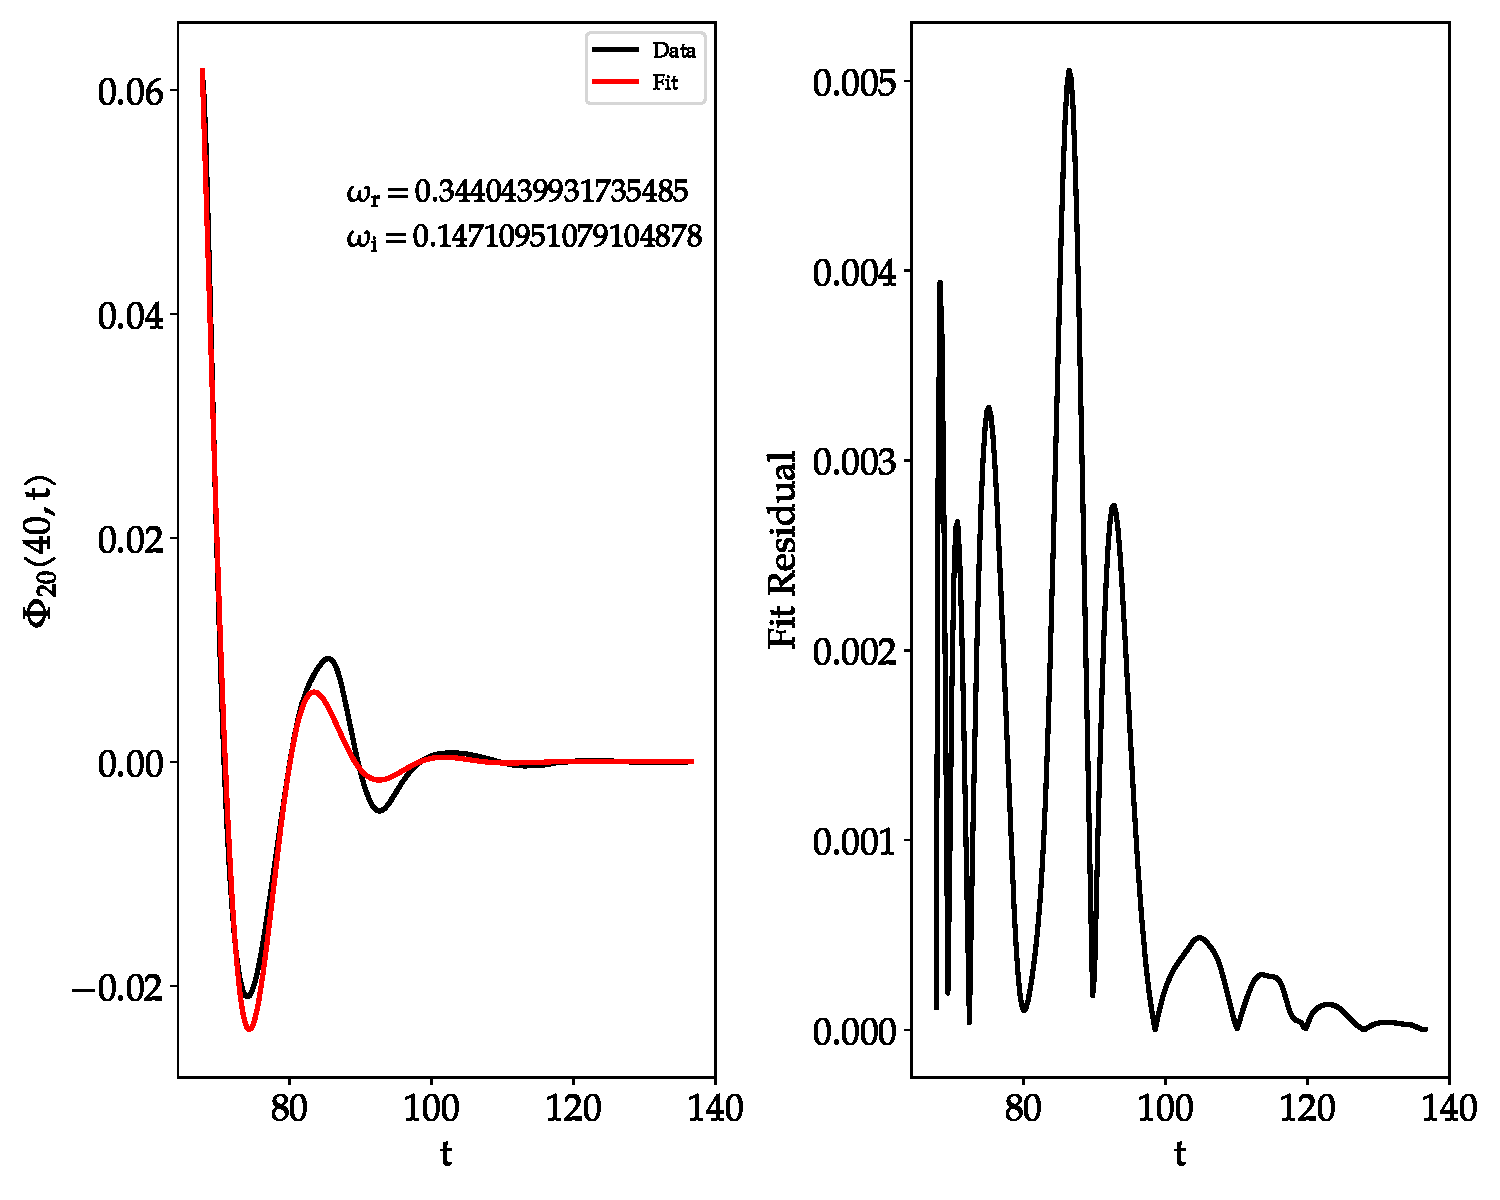
\includegraphics[width=\linewidth]{img/wave_scattering/fit_plot}
  \caption{Left panel: The original data is plotted against a fit to a quasinormal mode model. Fitted frequencies are displayed in the plot. Right panel: Plot of the absolute value of the difference between original and fitted data (fit residual). }
  \label{fig:multipolar_plots_fit}
\end{figure}

In conclusion, a spectral analysis of the signal has been conducted using the periodogram shown in Fig.~\ref{fig:multipolar_plots_psd}, which depicts the Power Spectral Density (PSD) of all frequency components in the simulated signal. The plot indicates a peak frequency at around $f\approx0.13$. Our aim in performing this analysis is to enhance the identification of oscillation frequencies in the signal in a more precise manner. Unlike approaches that rely on assumptions regarding the nature of the ringdown or starting times for model fitting, a periodogram analyzes all frequency components present in the signal.

\begin{figure}[h]
  \centering
  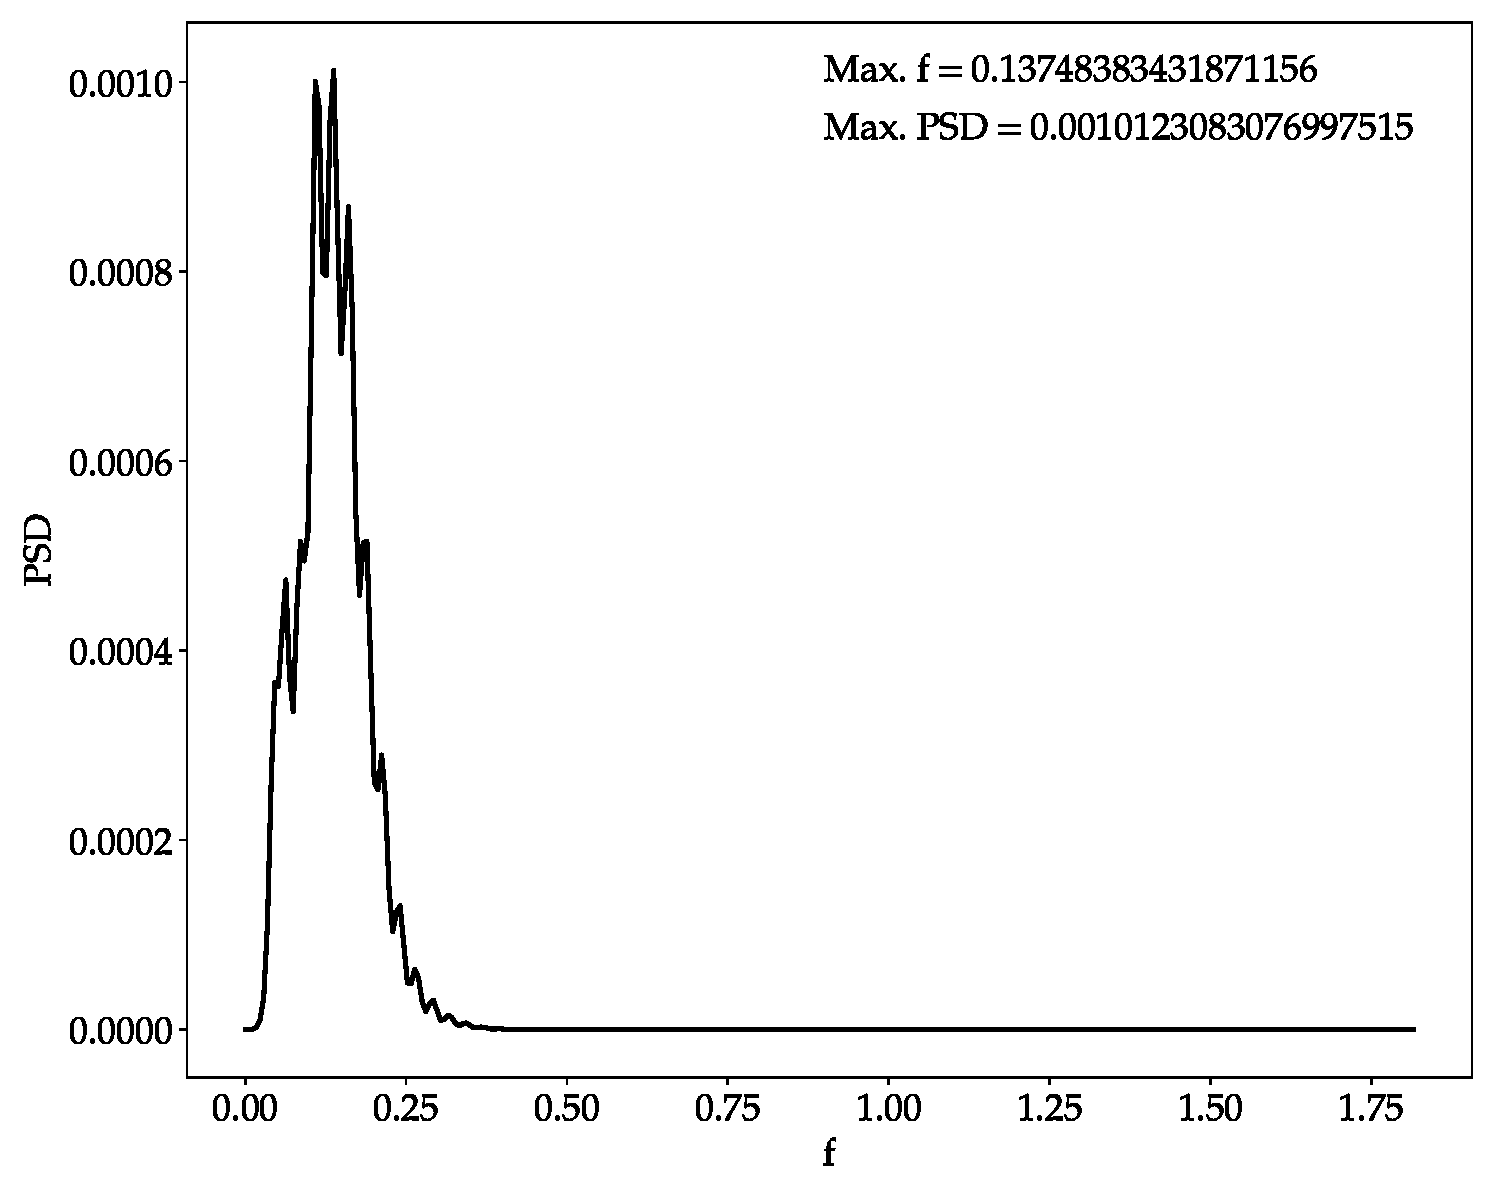
\includegraphics[width=\linewidth]{img/wave_scattering/psd_plot}
  \caption{Periodogram of the simulated signal with peak frequency indicated in the plot.}
  \label{fig:multipolar_plots_psd}
\end{figure}